%-----------------------------------
% Define document and include general packages
%-----------------------------------
\documentclass[12pt,oneside,titlepage,listof=totoc,bibliography=totoc]{scrartcl}
\usepackage[utf8]{inputenc}
\usepackage[ngerman]{babel}
\usepackage[babel,german=quotes]{csquotes}
\usepackage[T1]{fontenc}
\usepackage{fancyhdr}
\usepackage{fancybox}
\usepackage[a4paper, left=4cm, right=2cm, top=2.8cm, bottom=2.3cm]{geometry}
\usepackage{graphicx}
%\usepackage{svg}
\usepackage{colortbl}
\usepackage{array}
\usepackage{float}      %Positionierung von Abb. und Tabellen mit [H] erzwingen
\usepackage{footnote}
\usepackage{caption}
\usepackage{enumitem}
\usepackage{amssymb}
\usepackage{mathptmx}
\usepackage{amsmath}
\usepackage{xcolor}
\usepackage{marvosym}			% Verwendung von Symbolen, z.B. perfektes Eurozeichen
\usepackage[colorlinks=true,linkcolor=black]{hyperref}
\definecolor{darkblack}{rgb}{0,0,0}
\hypersetup{colorlinks=true, breaklinks=true, linkcolor=darkblack, menucolor=darkblack, urlcolor=darkblack}
\fontfamily{ptm}\selectfont

% Mehrere Fussnoten nacheinander mit Komma separiert
\usepackage[hang, multiple]{footmisc}
\setlength{\footnotemargin}{1em}

% todo Aufgaben als Kommentare verfassen für verschiedene Editoren
\usepackage{todonotes}

%Pakete für Tabellen
\usepackage{epstopdf}
\usepackage{nicefrac} % Brüche
\usepackage{multirow}
\usepackage{rotating} % vertikal schreiben
\usepackage{mdwlist}

\definecolor{dunkelgrau}{rgb}{0.8,0.8,0.8}
\definecolor{hellgrau}{rgb}{0.0,0.7,0.99}
% Colors for listings
\definecolor{mauve}{rgb}{0.58,0,0.82}
\definecolor{dkgreen}{rgb}{0,0.6,0}

% sauber formatierter Quelltext
\usepackage{listings}
\lstset{numbers=left,
	numberstyle=\tiny,
	numbersep=5pt,
	breaklines=true,
	showstringspaces=false,
	frame=l ,
	xleftmargin=5pt,
	xrightmargin=5pt,
	basicstyle=\ttfamily\scriptsize,
	stepnumber=1,
	keywordstyle=\color{blue},          % keyword style
  	commentstyle=\color{dkgreen},       % comment style
  	stringstyle=\color{mauve}         % string literal style
}

% Biblatex
\usepackage[
backend=biber,
style=numeric,
citestyle=authoryear,
url=false,
isbn=false,
notetype=footonly,
hyperref=false,
sortlocale=de]{biblatex}

%weitere Anpassungen für BibLaTex
% Opptionen für Biblatex
\ExecuteBibliographyOptions{%
giveninits=false,
isbn=true, 
url=true, 
doi=false, 
eprint=false,
maxbibnames=7, % Alle Autoren (kein et al.)
maxcitenames=2, % et al. ab dem 3. Autor
backref=false, % Rückverweise auf Zitatseiten
bibencoding=utf8, % wenn .bib in utf8, sonst ascii
bibwarn=true, % Warnung bei fehlerhafter bib-Datei
}%

% et al. an Stelle von u.a.
\DefineBibliographyStrings{ngerman}{ 
   andothers = {{et\,al\adddot}},             
}

% Klammern um das Jahr in der Fußnote
\renewbibmacro*{cite:labelyear+extrayear}{% 
  \iffieldundef{labelyear} 
    {} 
    {\printtext[bibhyperref]{% 
       \mkbibparens{% 
         \printfield{labelyear}% 
         \printfield{extrayear}}}}}

\DeclareNameFormat{last-first}{%
  \iffirstinits
    {\usebibmacro{name:family-given}
        {\namepartfamily}
        {\namepartgiveni}
        {\namepartprefix}
        {\namepartsuffix}
    }
    {\usebibmacro{name:family-given}
        {\namepartfamily}
        {\namepartgiven}
        {\namepartprefix}
        {\namepartsuffix}
    }%
  \usebibmacro{name:andothers}}

% Alternative Notation der Fußnoten 
% Zeigt sowohl den Nachnamen als auch den Vornamen an
% Beispiel: \fullfootcite[Vgl. ][Seite 5]{Tanenbaum.2003} 
\DeclareCiteCommand{\fullfootcite}[\mkbibfootnote]
  {\usebibmacro{prenote}}
  {\usebibmacro{citeindex}%
    \printnames[sortname][1-1]{author}%
    \addspace (\printfield{year})}
  {\addsemicolon\space}
  {\usebibmacro{postnote}}

%Autoren (Nachname, Vorname)
\DeclareNameAlias{default}{family-given}

%Reihenfolge von publisher, year, address verändern
% Achtung, bisher nur für den Typ @book definiert

%% Definiert @Book Eintrag
\DeclareBibliographyDriver{book}{%
  \printnames{author}%
  \newunit\addcolon\space
  \printfield{title}%
  \setunit*{,\space}%
  \printfield{edition}%
  \setunit*{\addcomma\space}%
  \printlist{publisher}%
  \newunit\newblockpunct
  \printlist{location}%
  \setunit*{\space}%
  \printfield{year}%
  \setunit*{,\space}% 
  \printfield{isbn}%
  \finentry}

%% Definiert @Online Eintrag
\DeclareBibliographyDriver{online}{%
  \printnames{author}%
  \newunit\newblockpunct
  \printfield{title}%
  \setunit*{,\space}%
  %\newunit\newblock
  \printfield{url}%
  \setunit*{,\space Erscheinungsjahr:\space}%
  \printfield{year}%
  \setunit*{,\space Aufruf am:\space}%
  \printfield{note}%
  \finentry}
  
%% Definiert @Article Eintrag
\DeclareBibliographyDriver{article}{%
	\printnames{author}%
	\newunit\newblockpunct
	\printfield{title}%
	\setunit*{.\space In:\space}%
	%\newunit\newblock
	\usebibmacro{journal}%
	\setunit*{\space (}%
	\printfield{year}\newunit{)}%
	\finentry}

%\DeclareBibliographyDriver{article}{%
%  \printnames{author}%
%  \newunit\newblockpunct
%  \printfield{title}%
%  \setunit*{.\space In:\space}%
%  %\newunit\newblock
%  \usebibmacro{journal}%
%  \setunit*{\space (}%
%  \printfield{year}\newunit{)}%
%  \finentry}

%% Definiert @InProceedings Eintrag
\DeclareBibliographyDriver{inproceedings}{%
	\printnames{author}%
	\setunit*{,\space (}%
	\printfield{year}\newunit{)}%
	\newunit\newblockpunct
	\printfield{title}%
	\setunit*{\space}%	
	\usebibmacro{booktitle}%
	\setunit*{,\space}%
	\printfield{isbn}%
	\setunit*{,\space}% 
	\printfield{doi}%
	\finentry}

%Doppelpunkt nach dem letzten Autor
\renewcommand*{\labelnamepunct}{\addcolon\addspace }

%Komma an Stelle des Punktes
\renewcommand*{\newunitpunct}{\addcomma\space}

%Autoren durch Semikolon trennen
\newcommand*{\bibmultinamedelim}{\addsemicolon\space}% 
\newcommand*{\bibfinalnamedelim}{\addsemicolon\space}% 
\AtBeginBibliography{% 
  \let\multinamedelim\bibmultinamedelim 
  \let\finalnamedelim\bibfinalnamedelim 
}

%Titel nicht kursiv anzeigen 
\DeclareFieldFormat{title}{#1\isdot}



%Bib-Datei einbinden
\addbibresource{literatur/Thesis.bib}

% Pfad fuer Abbildungen
\graphicspath{{./}{./abbildungen/}}

%-----------------------------------
% Weitere Ebene einfügen
\usepackage{titletoc}

\makeatletter

% Setze die Tiefe des Inhaltsverzeichnis auf 4 Ebenen
% Damit erscheinen \paragraph-Sektionen auch im Inhaltsverzeichnis
\setcounter{secnumdepth}{4}
\setcounter{tocdepth}{4}

% Fuege Abstand nach unten wie in einer normalen \section hinzu
% Andernfalls haette \paragraph keinen Zeilenumbruch
% Der Zeilenumbruch koennte mit einer leeren \mbox{} ersetzt werden
% Jedoch klebt dann der Text relativ nah an der Ueberschrift
\renewcommand{\paragraph}{%
  \@startsection{paragraph}{4}%
  {\z@}{3.25ex \@plus 1ex \@minus .2ex}{1.5ex plus 0.2ex}%
  {\normalfont\normalsize\bfseries\sffamily}%
}

\makeatother


%-----------------------------------
% Zeilenabstand 1,5-zeilig
%-----------------------------------
\usepackage{setspace}
\onehalfspacing

%-----------------------------------
% Absätze durch eine neue Zeile
%-----------------------------------
\setlength{\parindent}{0mm}
\setlength{\parskip}{0.8em plus 0.5em minus 0.3em}

\sloppy					%Abstände variieren
\pagestyle{headings}

%-----------------------------------
% Abkürzungsverzeichnis
%-----------------------------------
\usepackage[intoc]{nomencl}
\renewcommand{\nomname}{Abkürzungsverzeichnis}
\setlength{\nomlabelwidth}{.20\textwidth}
\renewcommand{\nomlabel}[1]{#1 \dotfill}
\setlength{\nomitemsep}{-\parsep}
\makenomenclature

%-----------------------------------
% Meta informationen
%-----------------------------------
%-----------------------------------
% Meta Informationen zur Arbeit
%-----------------------------------

% Autor
\newcommand{\myAutor}{Salih Komsucuk}

% Adresse
\newcommand{\myAdresse}{Grillostra\ss e 85 \\ \> \> 45881 Gelsenkirchen}

% Titel der Arbeit
\newcommand{\myTitel}{Diskrepanzen zwischen Technologietrends in Wirtschaft und Wissenschaft}

% Betreuer
\newcommand{\myBetreuer}{Fabian Gampfer}

% Lehrveranstaltung
\newcommand{\myLehrveranstaltung}{}

% Matrikelnummer
\newcommand{\myMatrikelNr}{328612}

% Ort
\newcommand{\myOrt}{Gelsenkirchen}

% Datum der Abgabe
\newcommand{\myAbgabeDatum}{\today}

% Semesterzahl
\newcommand{\mySemesterZahl}{7}

% Name der Hochschule
\newcommand{\myHochschulName}{FOM Hochschule für Oekonomie \& Management Essen}

% Standort der Hochschule
\newcommand{\myHochschulStandort}{Standort Essen}

% Studiengang
\newcommand{\myStudiengang}{Wirtschaftsinformatik}

% Art der Arbeit
\newcommand{\myThesisArt}{Exposé zur Bachelor Thesis}

% Zu erlangender akademische Grad
\newcommand{\myAkademischerGrad}{Bachelor of Science (B. Sc.)}

% Firma
\newcommand{\myFirma}{PSI Software AG}

%-----------------------------------
% PDF Meta Daten setzen
%-----------------------------------
\hypersetup{
    pdfinfo={
        Title={\myTitel},
        Subject={\myStudiengang},
        Author={\myAutor},
        Build=1.1
    }
}

%-----------------------------------
% Umlaute in Code korrekt darstellen
% siehe auch: https://en.wikibooks.org/wiki/LaTeX/Source_Code_Listings
%-----------------------------------
\lstset{literate=
	{á}{{\'a}}1 {é}{{\'e}}1 {í}{{\'i}}1 {ó}{{\'o}}1 {ú}{{\'u}}1
	{Á}{{\'A}}1 {É}{{\'E}}1 {Í}{{\'I}}1 {Ó}{{\'O}}1 {Ú}{{\'U}}1
	{à}{{\`a}}1 {è}{{\`e}}1 {ì}{{\`i}}1 {ò}{{\`o}}1 {ù}{{\`u}}1
	{À}{{\`A}}1 {È}{{\'E}}1 {Ì}{{\`I}}1 {Ò}{{\`O}}1 {Ù}{{\`U}}1
	{ä}{{\"a}}1 {ë}{{\"e}}1 {ï}{{\"i}}1 {ö}{{\"o}}1 {ü}{{\"u}}1
	{Ä}{{\"A}}1 {Ë}{{\"E}}1 {Ï}{{\"I}}1 {Ö}{{\"O}}1 {Ü}{{\"U}}1
	{â}{{\^a}}1 {ê}{{\^e}}1 {î}{{\^i}}1 {ô}{{\^o}}1 {û}{{\^u}}1
	{Â}{{\^A}}1 {Ê}{{\^E}}1 {Î}{{\^I}}1 {Ô}{{\^O}}1 {Û}{{\^U}}1
	{œ}{{\oe}}1 {Œ}{{\OE}}1 {æ}{{\ae}}1 {Æ}{{\AE}}1 {ß}{{\ss}}1
	{ű}{{\H{u}}}1 {Ű}{{\H{U}}}1 {ő}{{\H{o}}}1 {Ő}{{\H{O}}}1
	{ç}{{\c c}}1 {Ç}{{\c C}}1 {ø}{{\o}}1 {å}{{\r a}}1 {Å}{{\r A}}1
	{€}{{\EUR}}1 {£}{{\pounds}}1
}

%-----------------------------------
% Kopfbereich / Header definieren
%-----------------------------------
\pagestyle{fancy}
\fancyhf{}
\fancyhead[C]{-\ \thepage\ -}						% Seitenzahl oben, mittig
%\fancyhead[L]{\leftmark}							% kein Footer vorhanden
\renewcommand{\headrulewidth}{0.4pt}


%-----------------------------------
% Start the document here:
%-----------------------------------
\begin{document}

\pagenumbering{Roman}								% Seitennumerierung auf römisch umstellen
\renewcommand{\refname}{Literaturverzeichnis}		% "Literatur" in
%"Literaturverzeichnis" umbenennen
\newcolumntype{C}{>{\centering\arraybackslash}X}	% Neuer Tabellen-Spalten-Typ:
%Zentriert und umbrechbar

%-----------------------------------
% Titlepage
%-----------------------------------
\begin{titlepage}
	\newgeometry{left=2cm, right=2cm, top=2cm, bottom=2cm}
	\begin{center}
		\textbf{\myHochschulName}\\
		\textbf{\myHochschulStandort}\\
		\vspace{1.5cm}
			
\includegraphics[width=3cm]{abbildungen/fom.pdf} \\
		\vspace{1.5cm}
		Berufsbegleitender Studiengang\\
		\myStudiengang \\ %, \mySemesterZahl. Semester\\
		\vspace{2cm}
		\textbf{\myThesisArt}\\
		\textbf{zur Erlangung des Grades eines}\\
		\textbf{\myAkademischerGrad}\\
		% Oder für Hausarbeiten:
		%\textbf{im Rahmen der Lehrveranstaltung}\\
		%\textbf{\myLehrveranstaltung}\\
		\vspace{2cm}
		über das Thema\\
		\Huge{\myTitel}\\
		\vspace{0.2cm}
	\end{center}
	\normalsize
	\vfill
	\begin{tabbing}
		Links \= Mitte \= Rechts\kill
		Betreuer: \> \> \myBetreuer\\
		\> \> \\

		Autor: \> \> \myAutor\\
		\> \>  Matrikelnr.: \myMatrikelNr\\
%		\> \> \myAdresse\\
%		\> \> \\
		Abgabe: \> \> %\myAbgabeDatum
	\end{tabbing}
\end{titlepage}

%-------Ende Titelseite-------------

%-----------------------------------
% Sperrvermerk
%-----------------------------------
%\newpage
\thispagestyle{empty}

%-----------------------------------
% Sperrvermerk
%-----------------------------------
\section*{Sperrvermerk}
Die vorliegende Abschlussarbeit mit dem Titel \enquote{\myTitel} enthält unternehmensinterne Daten der Firma \myFirma . Daher ist sie nur zur Vorlage bei der FOM sowie den Begutachtern der Arbeit bestimmt. Für die Öffentlichkeit und dritte Personen darf sie nicht zugänglich sein.

\par\medskip
\par\medskip

\_\_\_\_\_\_\_\_\_\_\_\_\_\_\_\_\_\_\_\_\_\_\_\_ \hspace{1.5cm} \_\_\_\_\_\_\_\_\_\_\_\_\_\_\_\_\_\_\_\_\_\_\_\_ \\
(Ort, Datum)\hspace{4.5cm}
(Eigenhändige Unterschrift)

\newpage

%-----------------------------------
% Inhaltsverzeichnis
%-----------------------------------
\setcounter{page}{2}
\tableofcontents
\newpage

%-----------------------------------
% Abkürzungsverzeichnis
%-----------------------------------
\printnomenclature
\newpage
%-----------------------------------
% Abbildungsverzeichnis
%-----------------------------------
\listoffigures
\newpage
%-----------------------------------
% Tabellenverzeichnis
%-----------------------------------
\listoftables
\newpage
%-----------------------------------
% Seitennummerierung auf arabisch und ab 1 beginnend umstellen
%-----------------------------------
\pagenumbering{arabic}
\setcounter{page}{1}
%-----------------------------------
% Kapitel / Inhalte
%-----------------------------------
\section{Überlegungen zum Titel}

\section{Einleitung}
Die wissenschaftliche Forschung wurde als wichtiger Einflussfaktor für die Entstehung neuer Technologien und Technologietrends in bedeutenden Studien nachgewiesen.\footcite[Vgl.][S.~187]{Nelson1986}\footcite[Vgl.][S.~11]{Mansfield1991}\footcite[Vgl.][S.~599]{Tegarden2012} Nach Jaffe wird diese Erkenntnis bereits durch die geographische Nähe von Zentren der Spitzentechnologie wie das "`Silicon Valley"' oder die "`Massachusetts Route 128"' zu führenden Universitäten gestützt.\footcite[Vgl.][S.~967f]{Jaffe1989} Nach einer Studie von Mansfield wären etwa 11~\% aller Produkte einer Auswahl aus sieben Fertigungsindustrien im Betrachtungszeitraum gar nicht oder nur mit erheblicher Zeitverzögerung entwickelt worden, wäre dem nicht eine entsprechende wissenschaftliche Forschung vorausgegangen.\footcite[Vgl.][S.~2]{Mansfield1991}

Dennoch liegt die maßgebliche Entscheidung über den Einsatz und die Weiterentwicklung neuer Technologien vorwiegend in Händen von Unternehmern, Managern und sonstigen Entscheidungsträgern der praktizierenden Wirtschaft. Die wiederum richten ihre Entscheidungen unter Berücksichtigung einer Vielzahl von Faktoren an den Markt aus, um den Unternehmenserfolg zu steigern.\footcite[Vgl.][S.~1652f]{Gruber2008} Dabei greifen sie auch auf Informationsquellen von spezialisierten Unternehmen zurück, die mit Hilfe proprietärer Methoden Prognosen für Technologietrends in eigenen Publikationen herausgeben. Einer der einflussreichsten und bekanntesten Vertreter dessen ist der "`Gartner Hype Cycle"', den große Unternehmen bei strategischen Entscheidungen bezüglich neuer Technologien beratend hinzuziehen.\footcite[Vgl.][S.~254]{Steinert2010}

Nach Beyer ist der Einfluss auf Technologietrends durch Wirtschaftsmedien höher als durch wissenschaftliche Artikel, da sie von Managern aufgrund des gewohnten Fachjargons sowie der Praxisrelevanz bevorzugt gelesen werden.\footcite[Vgl.][S.~472]{Beyer1992} Barley et al. fanden sogar heraus, dass sich gängige Begriffe der Wirtschaft in wissenschaftlicher Literatur verzögert manifestieren, folglich der Einfluss unidirektional von Unternehmern in Richtung Akademiker stattfindet.\footcite[Vgl.][S.~52]{Barley1988} Nach Spell hängt das allerdings eher damit zusammen, dass wissenschaftliche Artikel einem Peer-Review unterzogen werden, welcher Monate bis Jahre in Anspruch nehmen kann, bis sie in Fachartikeln erscheinen, als dass wissenschaftliche Forschungsschwerpunkte stets aus Wirtschaftsjournalen gespeist würden. \footcite[Vgl.][S.~345]{Spell1999} 

\subsection{Problemstellung}
Somit findet eine gegenseitige Einflussnahme hinsichtlich der Prognose von Technologietrends zwischen Entscheidungsträgern der Wirtschaft und akademischen Forschern zweifelsohne statt. Gleichzeitig ist aufgrund teils unterschiedlicher Interessen beider Parteien eine Diskrepanz bei der Schwerpunktsetzung evident. 

Technologiethemen insbesondere in Informationstechnologien sind ständiger Veränderung unterworfen\footcite[Vgl.][S.~107f]{Chang2009}, wodurch eine permanente Auseinandersetzung mit Trendthemen für beide Seiten unumgänglich ist. Obwohl das "`Gartner Hype Cycle"' bei der Lösung dieser Herausforderung hohe Anerkennung in der Praxis genießt, bleibt es in der akademischen Forschung weitestgehend unberücksichtigt.\footcite[Vgl.][S.~241]{OLeary2008}\footcite[Vgl.][S.~12]{Jarvenpaa2008}

Folglich stellt sich heute erneut die Frage, ob und in welchem Ausmaß sich prognostizierte Technologietrends aus der wirtschaftlichen Praxis in wissenschaftlichen Fachartikel widerspiegeln.

\subsection{Zielsetzung}
Das vorrangige Ziel der Arbeit ist es, über einen definierten Zeitraum Technologiethemen mit der höchsten medialen Präsenz in der Wirtschaft zu erfassen und die Verteilung dieser Themen in wissenschaftlichen Fachartikeln im Verhältnis gegenüberzustellen.

Dazu wird eine Datenbasis der Trendthemen aus dem "`Gartner Hype Cycle for Emerging Technologies"' für die jeweiligen Jahre des ausgewählten Zeitraumes entnommen. Anschließend werden diese Daten in mehreren Datenbanken für wissenschaftliche Fachartikel im vergleichbaren Zeitraum gesucht, um sie schließlich mit Hilfe quantitativer Methoden miteinander zu vergleichen.

Als Ergebnis der Analyse wird die Erkenntnis angestrebt, mögliche Diskrepanzen beim Verständnis für vielversprechende Trends festzustellen. Durch die retrospektive Analyse vergangener Trendthemen können mit heutiger Betrachtung möglicherweise weitere Erkenntnisse hinsichtlich der Ursachen für Abweichungen gewonnen werden.

\section{Überlegungen zum Titel}
Unter der Annahme des vorweggenommenen Analyseergebnisses, dass signifikante Unterschiede zwischen Technologietrends in der Wirtschaft und Wissenschaft existieren, sind folgende Arbeitstitel möglich:
\begin{enumerate}
	\item Diskrepanzen beim Verständnis für Technologietrends zwischen der praktizierenden Wirtschaft und akademischen Forschung: Eine empirische Analyse auf Basis des "`Gartner Hype Cycle for Emerging Technologies"'
	\item Unterschiede in der Trendauffassung für neue Technologien in Informationsquellen der Wirtschaft und wissenschaftlichen Fachartikeln: Eine Analyse auf Basis des "`Gartner Hype Cyle for Emerging Technologies"'
\end{enumerate}

Sollte eine ergebnisneutrale Titelform präferiert sein, sind alternativ folgende Titel denkbar:
\begin{enumerate}
	\item Untersuchung von Technologietrends im "`Gartner Hype Cycle for Emerging Technologies"' im Vergleich mit wissenschaftlichen Fachartikeln
	\item Empirische Analyse von Diskrepanzen zwischen Technologietrends im "`Gartner Hype Cycle for Emerging Technologies"' und wissenschaftlichen Publikationen
\end{enumerate}


\section{Methodik}
Der "`Gartner Hype Cycle"' ist eine graphische Darstellung des üblicherweise zu beobachtenden Reifeprozesses einer neuen Technologie. In Abbildung \ref{fig:ghc} ist der Rohaufbau einer solchen Graphik mit unter anderem dem Kurvenverlauf sowie den fünf Stufen bis zur Produktivität zu sehen. Der sogenannte "`Peak of Inflated Expectations"' zeigt die Phase mit den größten, meist überzogenen Erwartungen an die Technologie, in der auch die Medienpräsenz am höchsten ist.\footcite[Vgl.][S.~3f]{Fenn2017}

\begin{figure}
	\centering
	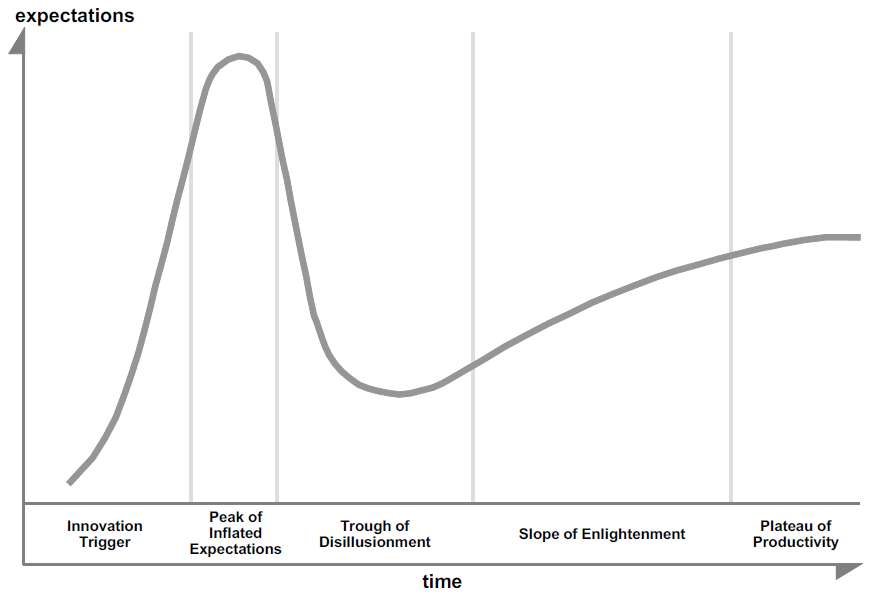
\includegraphics[width=0.9\linewidth]{abbildungen/ghc}
	\caption{Gartner Hype Cycle}
	\label{fig:ghc}
\end{figure}

Deshalb werden die hier aufgeführten Technologien der neusten Ausgabe als Grundlage für den Trendvergleich verwendet. Die letzte Publikation des 
"`Gartner Hype Cycle for Emerging Technologies"' ist im Juli 2017 erschienen und beinhaltet folgende chronologisch sortierte Technologien im Abschnitt "`Peak of Inflated Expectations"':\footcite[Vgl.][S.34-55]{Walker2017}
\begin{enumerate}
	\item Augmented Data Discovery
	\item Edge Computing
	\item Smart Robots
	\item IoT Platform
	\item Virtual Assistants
	\item Connected Home
	\item Deep Learning
	\item Machine Learning
	\item Autonomous Vehicles
	\item Nanotube Electronics
	\item Cognitive Computing
	\item Blockchain
	\item Commercial UAVs (Drones)
\end{enumerate}



Suchalgorithmen


mit Hilfe quantitativer Methoden
%\newpage
\section{Latex-Details}

\subsection{Verwendete Software, Editor und Zusatzpakete}
\subsubsection{Windows 8+}
\begin{itemize}
\item MikTex: 2.9, 32-bit
\item Biblatex: 3.5, Zusatz: Biber.exe
\item Editor: TexStudio (kann ich empfehlen), Notepad++
\end{itemize}

\subsubsection{Mac OSX und iOS}
\begin{itemize}
\item MacTeX: \url{https://tug.org/mactex}
\item Editor: TexPad \url{https://www.texpadapp.com}
\end{itemize}

\subsubsection{Online}
Overleaf ist eine Online-Anwendung mit der Ihr direkt im Browser an eurer Thesis schreiben könnt. Bis 1GB Größe und maximal 60 Einzeldateien könnt ihr Overleaf kostenlos nutzen: \url{https://www.overleaf.com/}


\subsection{Dokumentenklasse}
Eigentlich hatte Prof. Finke empfohlen die Dokumentklassen \enquote{Book} oder \enquote{Report} für die Erstellung der Bachelor-Thesis zu verwenden, da diese über weitere Gliederungsebenen verfügen. Ich verwende dennoch eine leicht modifizierte Komaskript-Klasse \enquote{scrartcl}, mit der Erweiterung um eine Ebene. Siehe (skripte/weitereEbene.tex). Das Skript stammt irgendwo aus den Netz und übersteigt meine \LaTeX{}-Fähigkeiten. Dadurch kann ich über eine weitere Ebene in der Arbeit verfügen, ohne mich mit der Modifikation von Kapitel-Seiten rumschlagen~\footcite[Vgl. ][Seite 5]{Tanenbaum.2003} zu müssen. Diese Quelle ist nur zur Demonstration und hat keinen inhaltlichen Bezug hierzu. Es werden übrigens nur die Quellen im Literaturverzeichnis angezeigt, die auch referenziert sind.


\subsection{Grafiken}
Das Paket \textbackslash usepackage\{float\} ermöglicht es die Grafiken und Tabellen an der Stelle im Text zu positionieren, wo diese im Quelltext stehen (Option H). Ansonsten würde \LaTeX{} diese dort unterbringen, wo es typographisch sinnvoll wäre - das wollen wir ja nicht ;-).

Die Breite der Grafiken am Besten relativ zum Text angeben.

\subsection{Quellcode}
Quellcode kann auf unterschiedliche Arten eingebaut werden.
Zum einen kann es hier durch direktives Einbinden in der Kapitel-Datei geschehen.
\begin{lstlisting}
% Hier wird aufgezeigt, wie man eine Grafik einbindet, es wird also in der PDF angezeigt,
% da es in einem Quellcode-Listing steht.
% Auch wenn es hier faelschlicherweise als LaTeX-Befehl angezeigt wird.
\includegraphics[width=0.9\textwidth]{sup}
\end{lstlisting}

Bei längeren Quellcode-Listings empfiehlt es sich jedoch auf eine externe Datei im Ordner Quellcode zu verlinken und diese einzubauen:
\lstinputlisting[language=HTML]{./Quellcode/Beispiel.html}

Da der Pfad zu den Abbildungen im Hauptdokument definiert wurde, muss hier nur noch der Name des Bildes ohne Dateiendung stehen (sup).


\begin{figure}[H]
\begin{center}
\includegraphics[width=0.9\textwidth]{sup}
\caption{Titel der Abbildung hier}
\end{center}
\end{figure}

\subsection{Tabellen}
\begin{table}[H]
\centering
\begin{tabular}[ht]{|l|l|l|}
  \hline
  \textbf{Abkürzung} & \textbf{Beschreibung} & \textbf{Berechnung}\\
  \hline\hline
    MEK & Materialeinzelkosten & \\
  	MGK & Materialgemeinkosten & $+ \uparrow$~*\\
    FEK & Fertigungseinzelkosten & \\
  	FGK & Fertigungsgemeinkosten & $+ \uparrow$~*\\
	SEKF & Sondereinzelkosten der Fertigung & \\
	\hline\hline
	\multicolumn{3}{|l|}{\textbf{= Herstellungskosten}} \\
	\hline\hline
  	VwGK & Verwaltungsgemeinkosten & $+ \uparrow$~*\\
  	VtGK & Vertriebsgemeinkosten & $+ \uparrow$~*\\
  	SEKVt & Sondereinzelkosten des Vertriebes & \\
	\hline\hline
	\multicolumn{3}{|l|}{\textbf{= Selbstkosten}} \\
	\hline\hline
	\multicolumn{3}{|l|}{+ Gewinnaufschlag} \\
	\multicolumn{3}{|l|}{+ Rabatte} \\
	\hline\hline
	\multicolumn{3}{|l|}{\textbf{= Nettoverkaufspreis (NVP)}} \\
	\hline
	\multicolumn{3}{|l|}{+ Umsatzsteuer} \\
	\hline\hline
	\multicolumn{3}{|l|}{\textbf{= Bruttoverkaufspreis (BVP)}} \\
	\hline
\end{tabular} \\
		\caption{Beispieltabelle 1}
		\label{tbl:beispieltabelle2}
\end{table}

%\clearpage % hiermit werden alle Bilder Tabellen ausgeworfen

\subsection{Biblatex}
Von den vielen verfügbaren Literatur-Paketen habe ich mich für Biblatex entschieden. Die Anforderungen der FOM sollten hiermit erfüllt sein. Ich habe bisher nur Einträge \enquote{@book} getestet. Wie immer steckt der Teufel hier im Detail und es wird sich später herausstellen, ob Biblatex eine gute Wahl war. Die Anpassungen hierfür liegen unter skripte/modsBiblatex. Ich verwende das Backend Biber, welches bib-Dateien in UTF-8 verarbeiten kann.

\subsection{Listen und Aufzählungen}
\subsubsection{Listen}
\begin{itemize}
\item ein wichtiger Punkt
\item noch ein wichtiger Punkt
\item und so weiter
\end{itemize}
\subsubsection{Aufzählungen}
\begin{enumerate}
\item Reihenfolge ist hier wichtig
\item Dieser Punkt kommt nach dem ersten
\item Da sollte jetzt eine 3 vorne stehen
\end{enumerate}

\paragraph{Tiefste Ebene 1}
Dies ist die tiefste Gliederungsebene. Sollten doch mehr Ebenen benötigt werden, muss eine andere Dokumentenklasse verwendet werden.

\paragraph{Tiefste Ebene 2}
Der zweite Punkt in dieser Ebene ist zur Erinnerung daran, dass es nie nie niemals nur einen Unterpunkt geben darf.

\subsection{Skript zum Kompilieren}
Latex will ja bekanntlich in einer bestimmten Reihenfolge aufgerufen werden:
\begin{lstlisting}
pdflatex thesis_main.tex
makeindex thesis_main.nlo -s nomencl.ist -o thesis_main.nls
biber thesis_main
pdflatex thesis_main.tex
pdflatex thesis_main.tex
thesis_main.pdf
\end{lstlisting}

Dies ist der Inhalt der Batchdatei \enquote{compile.bat}.

%\section{Fazit}
Wünsche Euch allen viel Erfolg für das 7. Semester und bei der Erstellung der Thesis. Über Anregungen und Verbesserung an dieser Vorlage würde ich mich sehr freuen. 

%-----------------------------------
% Literaturverzeichnis
%-----------------------------------
\newpage
%\addcontentsline{toc}{section}{Literatur}

\pagenumbering{Roman} %Zähler wieder römisch ausgeben
\setcounter{page}{4}  %Zähler manuell hochsetzen

\printbibliography

% Alternative Darstellung:
% Literaturverzeichnis nach Typ (@book, @arcticle ...) sortiert.
% Dazu die Zeile (\printbibliography) auskommentieren und folgenden code verwenden:

%\printbibheading
%\printbibliography[type=article,heading=subbibliography,title={Artikel}]
%\printbibliography[type=book,heading=subbibliography,title={Bücher}]
%\printbibliography[type=online,heading=subbibliography,title={Webseiten}]

\newpage
\fancyhead[C]{\thepage}
\pagenumbering{gobble} % Keine Seitenzahlen mehr

%-----------------------------------
% Ehrenwörtliche Erklärung
%-----------------------------------
\section*{Ehrenwörtliche Erklärung}
Hiermit versichere ich, dass die vorliegende Arbeit von mir selbstständig und ohne unerlaubte Hilfe angefertigt worden ist, insbesondere dass ich alle Stellen, die wörtlich oder annähernd wörtlich aus Veröffentlichungen entnommen sind, durch Zitate als solche gekennzeichnet habe. Ich versichere auch, dass die von mir eingereichte schriftliche Version mit der digitalen Version übereinstimmt. Weiterhin erkläre ich, dass die Arbeit in gleicher oder ähnlicher Form noch keiner Prüfungsbehörde / Prüfungsstelle vorgelegen hat. Ich erkläre mich damit einverstanden, dass die Arbeit der Öffentlichkeit zugänglich gemacht wird. Ich erkläre mich damit einverstanden, dass die Digitalversion dieser Arbeit zwecks Plagiatsprüfung auf die Server externer Anbieter hochgeladen werden darf. Die Plagiatsprüfung stellt keine Zurverfügungstellung für die Öffentlichkeit dar.


\vspace{5cm}

\begin{table}[h]
	\centering
	\begin{tabular*}{\textwidth}{c @{\extracolsep{\fill}} ccccc}
		Gelsenkirchen, \today
		&
		%PLACE YOUR SCANNED SIGNATURE INSIDE YOUR PICTURE DIRECTORY. CALL IT unterschrift.jpg
%		
\includegraphics[width=0.35\textwidth]{img/unterschrift}\vspace*{-0.35cm}
		\\
		\rule[0.5ex]{12em}{0.55pt} & \rule[0.5ex]{12em}{0.55pt} \\
		(Ort, Datum) & (Eigenhändige Unterschrift)
		\\
	\end{tabular*} \\
\end{table}

\end{document}
